\documentclass{beamer}

\usepackage{amsmath}
\usepackage{amssymb}
\usepackage{tikz}
\usepackage{pgfplots}

\title{Complex Eigenvalues}
\subtitle{\[A = PCP^{-1}\]}
\author{Ahmed Mohammed}
\institute{Georgia Institute of Technology}
\date{PLUS Session, Summer 2023}

\usetheme{Berlin}
\usefonttheme{serif}
\usecolortheme{crane}

\DeclareMathOperator{\re}{Re}
\DeclareMathOperator{\im}{Im}


\begin{document}
	\begin{frame}
		\maketitle
	\end{frame}

	\section{Open Activity}
	\begin{frame}
		\frametitle{Open Activity: Where We Left Off}
		Recall what the meaning of \emph{diagonalization} is. Remember what it means for a matrix to be \emph{similar}. \pause

		\begin{definition}
			A matrix \(A \in \mathbb{R}^{n \times n}\) is diagonalizable if and only if it is \textbf{similar} to a diagonal matrix.
		\end{definition}

		What if some of the eigenvalues of a real matrix are not only real, but with imaginary components?
	\end{frame}

	\begin{frame}
		\frametitle{Open Activity: Complex Numbers}
		Complex numbers are numbers that could be written in the form \(a + bi\), where \(a, b \in \mathbb{R}\). \pause
		
		If we wish, we can represent complex numbers as ``arrows" in a plane. For example, we can represent \(z = 3 + 2i\) as follows.
		\begin{figure}[!h]
			\centering
			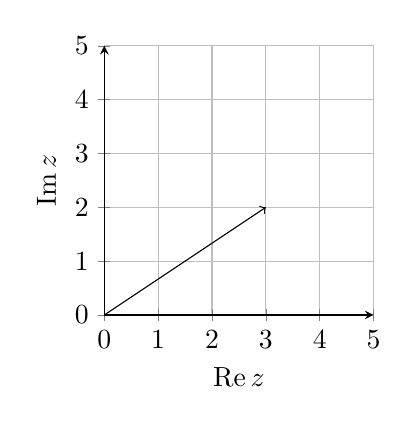
\begin{tikzpicture}
				\begin{axis}[axis lines=left, xmin=0, xmax=5, ymin=0, ymax=5, xtick distance=1, ytick distance=1, height=5cm, width=5cm, xlabel=\(\re z\), ylabel=\(\im z\), grid=major]
					\addplot[->, black] coordinates {(0, 0) (3, 2)};
				\end{axis}
			\end{tikzpicture}
		\end{figure}
	\end{frame}

	\begin{frame}
		\frametitle{Open Activity: Complex Numbers}
		Note that the arrow forms an angle with the (\(\re z\))-axis, and has a ``length" of \(\lvert 3 + 2i \rvert = \sqrt{3^2 + 2^2} = \sqrt{13}\).
		
		\begin{figure}[!h]
			\centering
			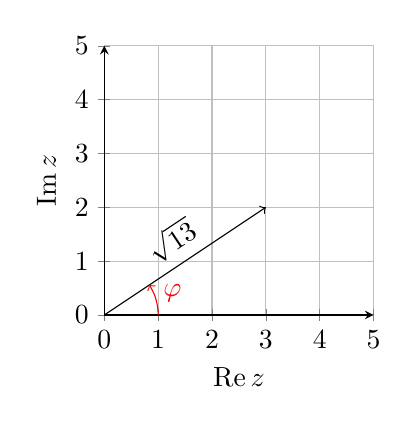
\begin{tikzpicture}
				\begin{axis}[axis lines=left, xmin=0, xmax=5, ymin=0, ymax=5, xtick distance=1, ytick distance=1, height=5cm, width=5cm, xlabel=\(\re z\), ylabel=\(\im z\), grid=major]
					\addplot[->, black] coordinates {(0, 0) (3, 2)} node[midway, above, sloped] {\(\small \sqrt{13}\)};
					\draw[red, ->] (axis cs: 1,0) arc (0:33.6:0.7cm) node[pos=0.7, right] {\(\varphi\)};
				\end{axis}
			\end{tikzpicture}
		\end{figure}
	\end{frame}

	\begin{frame}
		\frametitle{Open Activity: Complex Numbers (\textit{Cont.})}
		If we multiply two complex numbers \(z_1, z_2\) together, then we get another complex number \(z_3\) that makes an angle of 
		\(\varphi_{z_1} + \varphi_{z_2}\) with a length of \(\lvert z_1 \rvert \lvert z_2 \rvert\).

		\begin{figure}[!h]
			\centering
			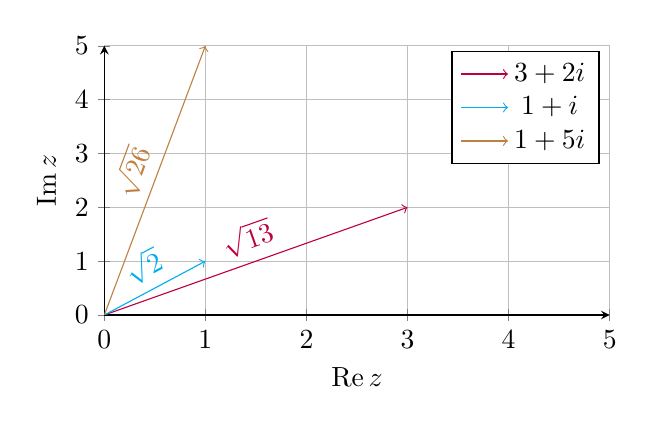
\begin{tikzpicture}
				\begin{axis}[axis lines=left, xmin=0, xmax=5, ymin=0, ymax=5, xtick distance=1, ytick distance=1, height=5cm, width=8cm, xlabel=\(\re z\), ylabel=\(\im z\), grid=major]
					\addplot[->, purple] coordinates {(0, 0) (3, 2)} node[midway, above, sloped] {\(\small \sqrt{13}\)};
					\addlegendentry{\(3 + 2i\)};
					\addplot[->, cyan] coordinates {(0, 0) (1, 1)} node[midway, above, sloped] {\(\small \sqrt{2}\)};
					\addlegendentry{\(1 + i\)};
					\addplot[->, brown] coordinates {(0, 0) (1, 5)} node[midway, above, sloped] {\(\small \sqrt{26}\)};
					\addlegendentry{\(1 + 5i\)};
				\end{axis}
			\end{tikzpicture}
		\end{figure}
	\end{frame}

	\begin{frame}
		\frametitle{Open Activity: Complex Numbers (\textit{Cont.})}
		Note that essentially what happened is that one of the numbers got \emph{rotated} then \emph{scaled}. Both of those are linear transformations. 
		What matrix represents their composition? \pause
		\begin{itemize}
			\item<2-> If we represented every complex numbers \(c + di\) as the vector \(\begin{bmatrix}c \\ d\end{bmatrix}\);
			\item<3-> and represented the operation of \emph{multiplication} with a complex number \(a + bi\) as \(\begin{bmatrix}a & -b \\ b & a\end{bmatrix}\begin{bmatrix}c \\ d\end{bmatrix}\),
		\end{itemize}
		\onslide<4>{We ``represent" complex number multiplication! Try it with the previous two examples. Set \(a + bi = 3 + 2i\) and try for the two 
		different complex numbers.}
	\end{frame}

	\begin{frame}
		\frametitle{The Last Intuitive Idea}
		We've discovered that the matrix \(\begin{bmatrix}a & -b \\ b & a\end{bmatrix}\) allows us to think about multiplying complex numbers. We've also
		discovered that it corresponds to a rotation and dilation, so every matrix in this form is called a rotation-dilation matrix. \pause

		What are the eigenvalues of matrices in this form? \pause
		Do the complex eigen-stuff come in pair?
	\end{frame}

	\begin{frame}
		\frametitle{Open Activity: Conclusion}
		Since matrices with the same eigenvalues are similar, any real \(2 \times 2\) matrix with complex eigenvalues must be similar to a rotation-dilation 
		matrix. That is, for any real \(2 \times 2\) matrix \(A\) with complex eigenvalues, it must be the case that there exists a \(P\) such that 
		\[A = PCP^{-1},\] where \(C\) is the corresponding rotation-dilation matrix, and \(P = \begin{bmatrix}\re \vec{v} & \im \vec{v}\end{bmatrix}\). 
		\(\vec{v}\) is a complex eigenvector of \(A\) living in \(\mathbb{C}^2\).
	\end{frame}

	\section{Main Activity: Examples}	
	\begin{frame}
		\begin{itemize}
			\item<1-> If \(A = \begin{bmatrix}\sqrt{3} & -1 \\ 1 & \sqrt{3}\end{bmatrix}\), then \(A\) is a rotation-dilation matrix. Find the scaling and angle of
				rotation for the transformation defined as \(A\vec{x} \mapsto \vec{x}\).
			\item<2-> Do the same for the matrix \(\begin{bmatrix}-\sqrt{3}/2 & 1/2\\ -1/2 & -\sqrt{3}/2\end{bmatrix}\).
			\item<3-> Find the corresponding \(C\) and \(P\) for the matrix \(A\) such that \(A = PCP^{-1}\).
				\begin{enumerate}
					\item<4-> \(\begin{bmatrix}1 & -2 \\ 1 & 3\end{bmatrix}\).
					\item<5-> \(\begin{bmatrix}1 & 5 \\ -2 & 3\end{bmatrix}\).
				\end{enumerate}
			\item<6-> Is it possible that a \(5 \times 5\) matrix has 3 complex eigenvalues and 2 real eigenvalues?
			\item<7-> Is it possible that a \(5 \times 5\) matrix has 3 complex eigenvectors and 3 real eigenvectors? 
		\end{itemize}
	\end{frame}
\end{document}
